\chapter{CRIAÇÃO DOS AMBIENTES DE DESENVOLVIMENTO}

\section{Introdução}

Este capítulo aborda o processo de criação e configuração dos ambientes e infraestruturas
necessárias para o desenvolvimento do protótipo de aplicação, incluindo o repositório no GitHub,
configuração do NestJS para monorepo, e a criação dos containers Docker e Docker Compose.
Cada uma dessas etapas é detalhada, com foco em suas contribuições para a construção de uma
arquitetura de micro serviços e mensageria, conforme modelado pelo C4 Model.

\section{Configuração do Supabase}

Conforme mencionado anteriormente, o Supabase é uma plataforma open-source que
simplifica a criação e gestão de componentes relacionados a bancos de dados e autenticação.
Ao iniciar um projeto, o Supabase configura automaticamente um banco de dados PostgreSQL
como estrutura base.

Adicionalmente, a plataforma oferece suporte à Row Level Security (RLS), que além de
assegurar a autenticação dos usuários, possibilita a configuração de autorizações, determinando
o nível de acesso (roles) de cada usuário conforme sua função ou permissão.
Outra grande vantagem sobre o Supabase, é a facilidade, pois para criar um projeto com
eles, podemos apenas acessar o link (https://supabase.com).

Um exemplo de criação de um projeto utilizando supabase:

\begin{figure}[!ht]
    \centering
    \caption{Criando o projeto no Supabase}
    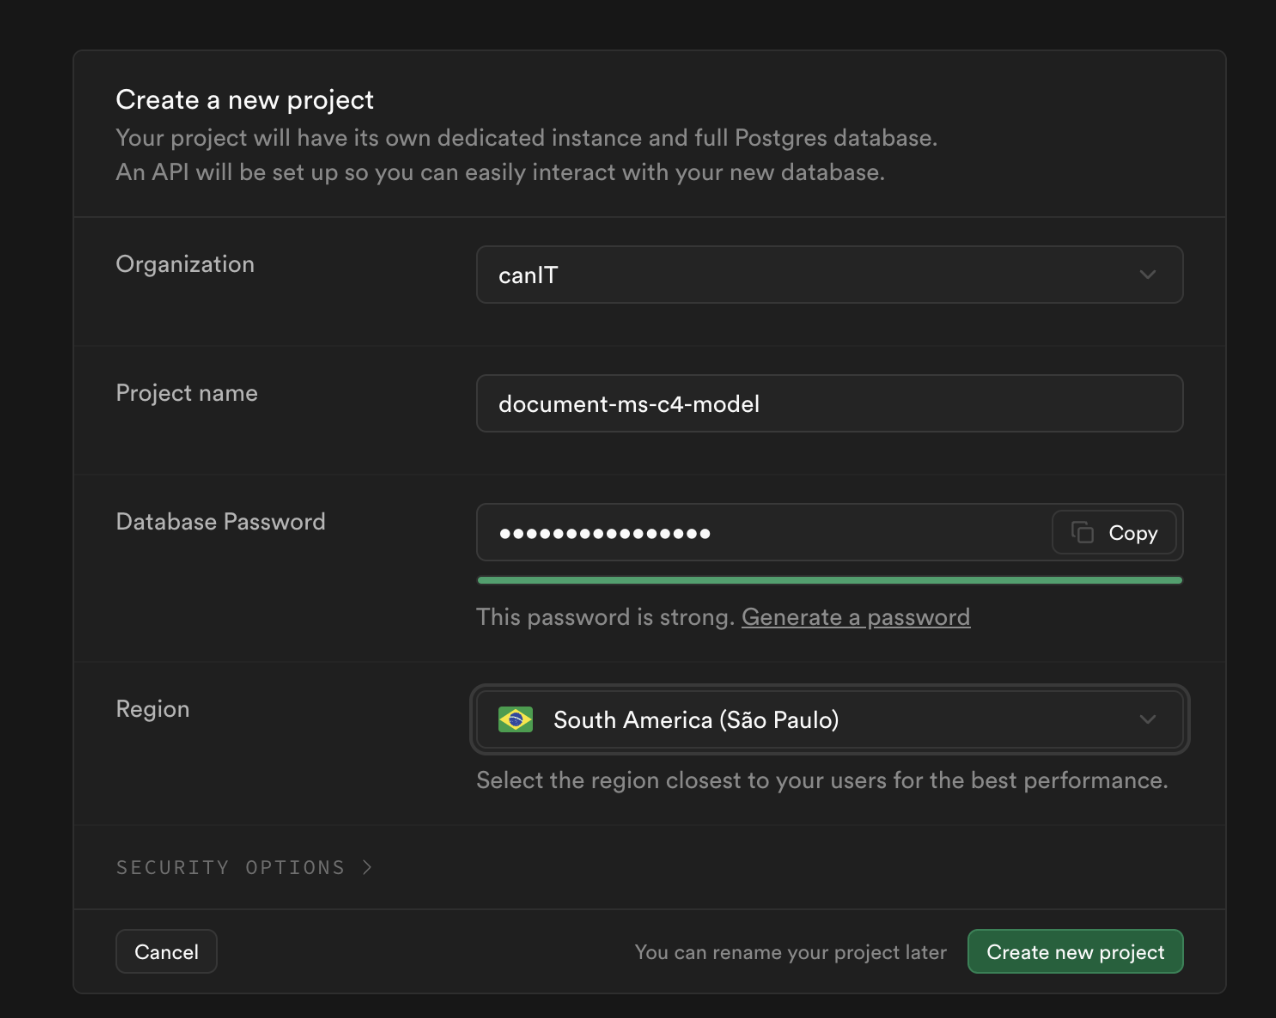
\includegraphics[scale=0.44]{assets/create-new-project}
    \label{fig:create-new-project}
    \tiny
    \sourcemedaddy
\end{figure}

Após a criação, temos um período de configuração, costuma demorar menos que 5
minutos, é redirecionado para essa página:

\begin{figure}[!ht]
    \centering
    \caption{Pendente de criação}
    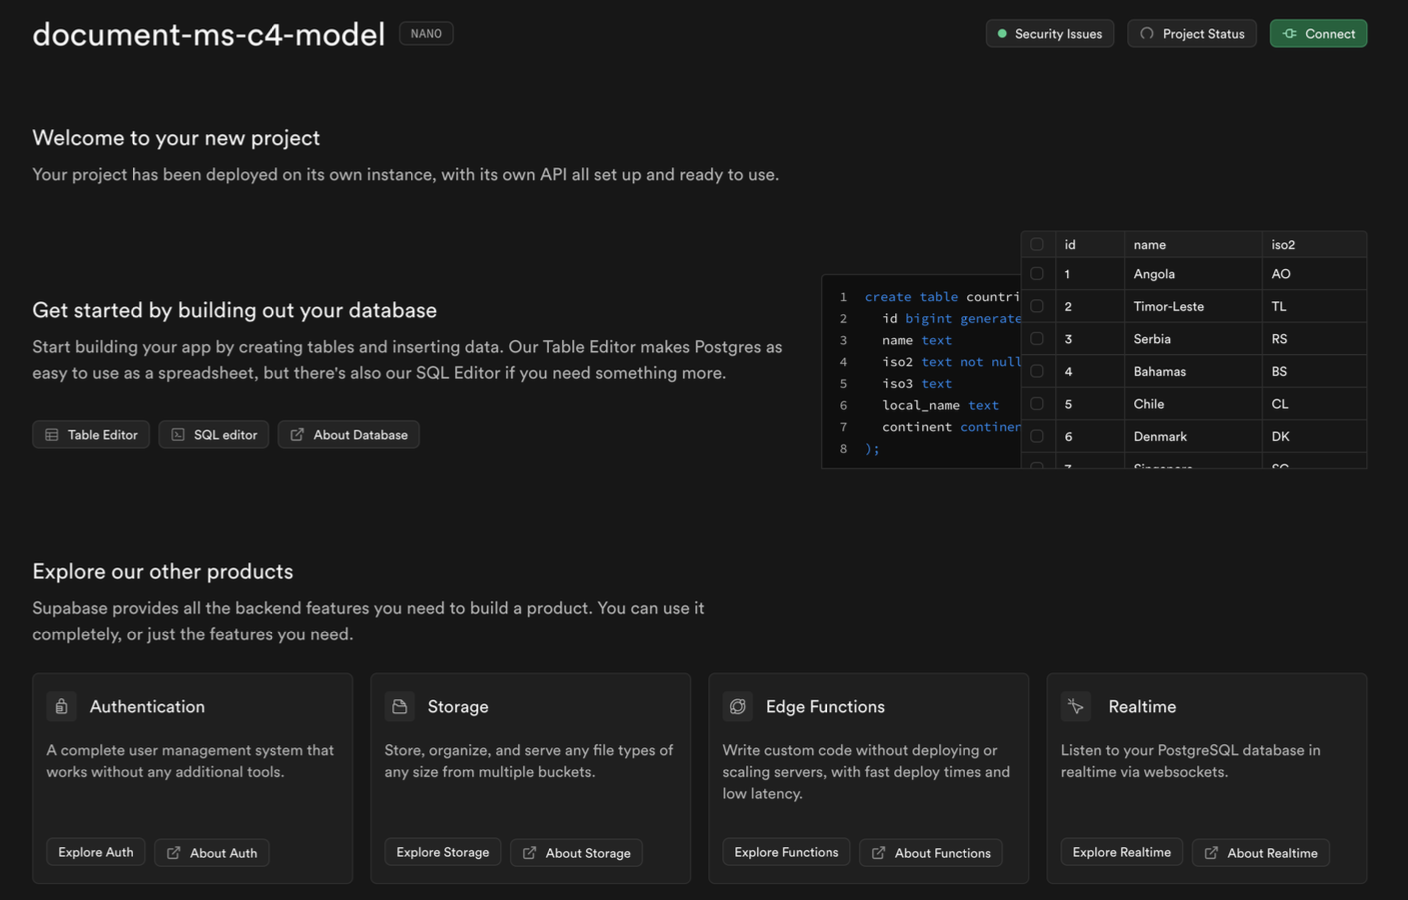
\includegraphics[scale=0.44]{assets/pending-creation}
    \label{fig:pending-creation}
    \tiny
    \sourcemedaddy
\end{figure}

Primeiro usuário criado no painel do Supabase:

\begin{figure}[!ht]
    \centering
    \caption{Pendente de criação}
    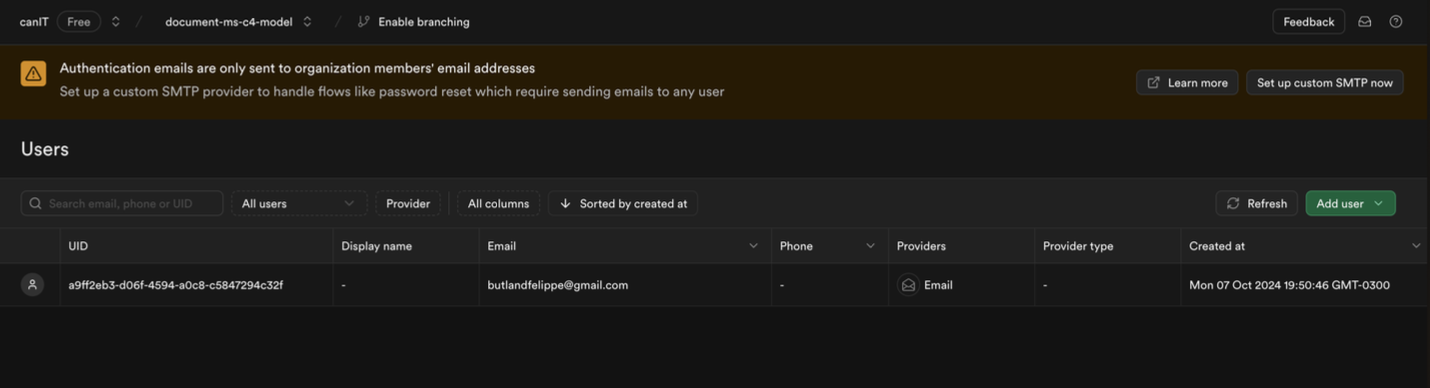
\includegraphics[scale=0.44]{assets/first-user}
    \label{fig:first-user}
    \tiny
    \sourcemedaddy
\end{figure}

\section{Criação de Repositório no GitHub}

A primeira etapa no processo de desenvolvimento é a criação do repositório onde o código-fonte será armazenado e versionado. O GitHub foi escolhido como plataforma de controle de versões, pois oferece integração com diversas ferramentas de CI/CD e uma ampla comunidade de desenvolvedores. A seguir estão os passos para a criação do repositório:

\begin{enumerate}
    \item Acesse o GitHub e faça login com suas credenciais.
    \item No canto superior direito da página inicial, clique em “+” e selecione a opção "New repository".
    \item Preencha as informações do repositório:
    \begin{itemize}
        \item \textbf{Repository name:} Nome do repositório (ex: "document-sharing-microservices").
        \item \textbf{Description:} Descrição breve do repositório (ex: "Protótipo de aplicação de envio de documentos modelado com C4, utilizando micro serviços e mensageria.").
        \item \textbf{Public/Private:} Selecione se o repositório será público ou privado.
        \item \textbf{Initialize this repository with:} Marque a opção "Add a README file" para inicializar o repositório com um arquivo README.
    \end{itemize}
    \item Clique em “Create repository”.
\end{enumerate}

Após a criação do repositório, o código fonte poderá ser versionado e colaborado com outras equipes utilizando Git.

\section{Configuração do NestJS para Monorepo e API Gateway}

O NestJS é um framework para desenvolvimento de aplicações backend utilizando Node.js e TypeScript. Para este projeto, a configuração de um monorepo utilizando NestJS facilita o gerenciamento de múltiplos micro serviços em uma única base de código, proporcionando escalabilidade e modularidade. Além disso, um API Gateway foi desenvolvido para atuar como a entrada centralizada para as requisições direcionadas aos diferentes micro serviços. O uso do API Gateway simplifica a comunicação entre o cliente e os serviços, permitindo uma melhor organização e gestão das requisições.

\subsection{Configuração do Monorepo}
Os passos para a configuração do monorepo são os seguintes:

\begin{enumerate}
    \item Instale o NestJS CLI globalmente utilizando o comando:
    \begin{verbatim}
    npm i -g @nestjs/cli
    \end{verbatim}
    \item Crie um novo projeto NestJS com suporte a monorepo, utilizando o comando:
    \begin{verbatim}
    nest new project-name --monorepo
    \end{verbatim}
    \item Durante a criação, selecione as opções desejadas para o gerenciamento de pacotes e outros aspectos do projeto.
    \item Navegue até o diretório do projeto e verifique a estrutura de pastas. O NestJS criará uma estrutura base contendo a pasta \texttt{apps}, que armazenará os micro serviços, e a pasta \texttt{libs}, que conterá os módulos compartilhados entre os micro serviços.
    \item Crie um novo micro serviço com o comando:
    \begin{verbatim}
    nest generate app microservice-name
    \end{verbatim}
    \item Para garantir que os micro serviços estejam corretamente configurados, execute o comando:
    \begin{verbatim}
    npm run start:dev
    \end{verbatim}
    Este comando iniciará o serviço em ambiente de desenvolvimento.
\end{enumerate}

\subsection{Desenvolvimento do API Gateway}
Para atuar como a entrada centralizada para as requisições, o API Gateway foi implementado no mesmo monorepo. Os passos para a configuração do API Gateway são os seguintes:

\begin{enumerate}
    \item Navegue até o diretório do projeto e crie uma nova aplicação para o API Gateway:
    \begin{verbatim}
    nest generate app api-gateway
    \end{verbatim}
    \item Instale as dependências necessárias, como o \texttt{@nestjs/microservices} para habilitar a comunicação entre micro serviços.
    \item Configure os controladores no API Gateway para encaminhar as requisições para os serviços apropriados. Utilize decorators como \texttt{@Get()}, \texttt{@Post()} etc., para definir as rotas.
    \item Implemente a lógica de balanceamento de carga, se necessário, utilizando a biblioteca \texttt{@nestjs/microservices} para garantir que as requisições sejam distribuídas de forma equitativa entre instâncias de micro serviços.
\end{enumerate}

\subsection{Suporte à Escalabilidade}
O API Gateway proporciona escalabilidade de diversas maneiras:

\begin{itemize}
    \item \textbf{Balanceamento de Carga}: Permite distribuir as requisições entre várias instâncias de um micro serviço, evitando sobrecargas e melhorando a disponibilidade.

    \item \textbf{Roteamento Dinâmico}: Facilita a adição ou remoção de serviços, permitindo que novos recursos sejam acessados rapidamente sem a necessidade de alterar a lógica de roteamento.

    \item \textbf{Escalabilidade Horizontal}: Cada micro serviço pode ser escalado independentemente, permitindo que a infraestrutura cresça conforme a demanda sem impactar os demais serviços.
\end{itemize}

\subsection{Considerações Finais}
A configuração do NestJS em um monorepo e a implementação do API Gateway proporcionam uma base sólida para o desenvolvimento de aplicações escaláveis e modulares. Essa arquitetura não apenas melhora a comunicação entre os micro serviços, mas também oferece flexibilidade para a adaptação a mudanças nas necessidades do negócio. A integração do API Gateway garante que o sistema possa crescer de forma organizada, permitindo uma resposta ágil às demandas do mercado e dos usuários.

\section{Criação do Docker e Docker Compose}

O Docker é utilizado para empacotar as aplicações em containers, garantindo consistência entre os ambientes de desenvolvimento e produção. O Docker Compose permite orquestrar múltiplos containers, facilitando a comunicação entre os micro serviços e o banco de dados. Para configurar o Docker e o Docker Compose para este projeto, siga os passos abaixo:

\subsection{Criação do Dockerfile}
Cada micro serviço criado no NestJS precisará de um arquivo Dockerfile para definir como o container será construído. O exemplo a seguir mostra a configuração básica de um Dockerfile para um micro serviço NestJS:

\begin{verbatim}
FROM node:16
WORKDIR /usr/src/app
COPY package*.json ./
RUN npm install
COPY . .
EXPOSE 3000
CMD ["npm", "run", "start:prod"]
\end{verbatim}

\subsection{Criação do docker-compose.yml}
O arquivo \texttt{docker-compose.yml} será utilizado para definir e orquestrar os containers dos micro serviços e dos componentes auxiliares, como bancos de dados e filas de mensagens. Um exemplo básico de configuração para o Docker Compose é apresentado a seguir:

\begin{verbatim}
version: '3.8'
services:
  kafka:
    image: confluentinc/cp-kafka:latest
    depends_on:
      - zookeeper
    ports:
      - 29092:29092
    environment:
      KAFKA_BROKER_ID: 1
      KAFKA_ZOOKEEPER_CONNECT: zookeeper:2181
      KAFKA_ADVERTISED_LISTENERS: PLAINTEXT://kafka:9092
      KAFKA_INTER_BROKER_LISTENER_NAME: PLAINTEXT
      KAFKA_OFFSETS_TOPIC_REPLICATION_FACTOR: 1
  kafka_ui:
    image: provectuslabs/kafka-ui:latest
    depends_on:
      - kafka
    ports:
      - 8080:8080
    environment:
      KAFKA_CLUSTERS_0_ZOOKEEPER: zookeeper:2181
      KAFKA_CLUSTERS_0_NAME: local
      KAFKA_CLUSTERS_0_BOOTSTRAPSERVERS: kafka:9092
volumes:
  mongodb_data_container:
\end{verbatim}

Este arquivo define o serviço da aplicação e do Kafka.

\subsection{Desafios de Rede com Docker}

Um dos principais desafios ao usar o Docker em um ambiente onde o banco de dados Supabase está localizado em uma rede diferente da rede Docker é a comunicação entre os containers e o banco de dados externo. Aqui estão alguns problemas que surgiram durante a configuração e as soluções aplicadas:

\begin{itemize}
    \item \textbf{Conectividade de Rede}: Inicialmente, os micro serviços não conseguiam se conectar ao Supabase devido à falta de configuração das variáveis de ambiente que definem as credenciais e a URL do banco de dados. A solução foi garantir que cada serviço no Docker recebesse as variáveis de ambiente corretas, utilizando o arquivo \texttt{docker-compose.yml} para passar essas informações, por exemplo:
    \begin{verbatim}
    environment:
      SUPABASE_URL: <url_do_supabase>
      SUPABASE_ANON_KEY: <chave_anonima>
    \end{verbatim}

    \item \textbf{Configuração de Redes Docker}: A comunicação entre os micro serviços e as filas de mensagens, como o Kafka, também apresentou dificuldades. Para resolver isso, foi criada uma rede personalizada no Docker Compose, permitindo que os serviços se comunicarem entre si e com o Supabase. A configuração foi realizada da seguinte forma:
    \begin{verbatim}
    networks:
      app-network:
        driver: bridge
    \end{verbatim}

    E cada serviço foi adicionado a esta rede:
    \begin{verbatim}
    services:
      kafka:
        networks:
          - app-network
      microservice:
        networks:
          - app-network
    \end{verbatim}

    \item \textbf{Latência de Rede}: A comunicação entre os containers e o Supabase pode introduzir latência, especialmente sob alta carga de tráfego. Foi implementado um mecanismo de retry e timeouts nas requisições feitas ao banco, garantindo que as operações críticas fossem executadas mesmo diante de instabilidades temporárias.

    \item \textbf{Perda de Conexões}: Em situações de reinicialização de containers, houve momentos em que as conexões com o banco de dados foram perdidas. Para mitigar esse problema, foi utilizado um padrão de reconexão automática nos micro serviços, que tentam reconectar-se ao Supabase até que a conexão seja restabelecida.
\end{itemize}

Esses desafios exigem uma configuração cuidadosa da rede e testes rigorosos para garantir que a comunicação entre os micro serviços e o Supabase seja confiável e eficiente. A implementação de práticas de robustez, como retries e configuração de variáveis de ambiente, ajudou a minimizar problemas de conectividade e latência, garantindo que o sistema como um todo funcione conforme o esperado.

\section{Configuração do Kafka e Zookeeper}

O Apache Kafka é uma plataforma de streaming de eventos que permite a construção de pipelines de dados em tempo real e aplicações de streaming. Para o funcionamento adequado do Kafka, é necessário o uso do Zookeeper, que é responsável por gerenciar a configuração do Kafka e o estado dos brokers. A configuração correta de ambos é essencial para garantir a resiliência e o desempenho do sistema. Abaixo, detalharemos a configuração dos serviços Kafka e Zookeeper, bem como os problemas comuns relacionados à latência e à perda de mensagens.

\subsection{Configuração do Zookeeper}
O Zookeeper deve ser configurado adequadamente para garantir que o Kafka funcione corretamente. No arquivo \texttt{docker-compose.yml}, o Zookeeper pode ser definido como um serviço separado, conforme exemplificado abaixo:

\begin{verbatim}
  zookeeper:
    image: wurstmeister/zookeeper:3.4.6
    ports:
      - 2181:2181
    environment:
      ZOOKEEPER_CLIENT_PORT: 2181
      ZOOKEEPER_TICK_TIME: 2000
\end{verbatim}

O parâmetro \texttt{ZOOKEEPER\_TICK\_TIME} define a frequência com que o Zookeeper envia notificações aos seus clientes e deve ser ajustado conforme a necessidade do sistema.

\subsection{Configuração do Kafka}
No arquivo \texttt{docker-compose.yml}, o Kafka é configurado para se conectar ao Zookeeper e definir as opções de replicação e comunicação entre brokers. A configuração apresentada anteriormente inclui as seguintes variáveis de ambiente:

\begin{verbatim}
  KAFKA_ZOOKEEPER_CONNECT: zookeeper:2181
  KAFKA_ADVERTISED_LISTENERS: PLAINTEXT://kafka:9092
  KAFKA_INTER_BROKER_LISTENER_NAME: PLAINTEXT
  KAFKA_OFFSETS_TOPIC_REPLICATION_FACTOR: 1
\end{verbatim}

- \textbf{KAFKA\_ZOOKEEPER\_CONNECT:} Define a conexão do Kafka com o Zookeeper.
- \textbf{KAFKA\_ADVERTISED\_LISTENERS:} Especifica os listeners disponíveis para os clientes se conectarem.
- \textbf{KAFKA\_INTER\_BROKER\_LISTENER\_NAME:} Determina o listener a ser usado para a comunicação entre brokers.
- \textbf{KAFKA\_OFFSETS\_TOPIC\_REPLICATION\_FACTOR:} Define o fator de replicação dos tópicos de offsets, que deve ser maior que 1 em produção para garantir alta disponibilidade.

\subsection{Problemas de Latência}
Um dos desafios ao trabalhar com Kafka é a latência. A latência pode ser causada por diversos fatores, como a configuração inadequada do número de partições, a replicação excessiva de dados ou a largura de banda insuficiente. Para mitigar a latência, recomenda-se:

\begin{itemize}
    \item Otimizar o número de partições para permitir um balanceamento adequado de carga.
    \item Ajustar as configurações de flush e a quantidade de memória disponível para o Kafka.
    \item Monitorar a rede e a infraestrutura para identificar gargalos.
\end{itemize}

\subsection{Perda de Mensagens}
A perda de mensagens é outro problema crítico em sistemas que utilizam Kafka. Isso pode ocorrer devido a configurações de replicação inadequadas ou falhas de broker. Para minimizar o risco de perda de mensagens, as seguintes práticas são recomendadas:

\begin{itemize}
    \item Configurar o fator de replicação dos tópicos para um valor maior que 1.
    \item Usar o modo de produção \texttt{acks=all} para garantir que todas as réplicas confirmem a gravação antes de considerar a mensagem como recebida.
    \item Implementar um sistema de monitoramento para detectar falhas rapidamente e garantir a recuperação adequada.
\end{itemize}

A correta configuração do Kafka e do Zookeeper, juntamente com a consideração dos problemas de latência e perda de mensagens, é essencial para garantir um sistema robusto e confiável de micro serviços.

\section{Arquitetura de Micro Serviços e Mensageria}

Neste projeto, a arquitetura de micro serviços é baseada em múltiplos serviços indepen-
dentes que se comunicam por meio de eventos assíncronos utilizando mensageria. A solução
de mensageria escolhida foi Kafka, adequado para sistemas que requerem alta escalabilidade e
comunicação entre serviços desacoplados.

A comunicação entre micro serviços será modelada utilizando o C4 Model, uma aborda-
gem que divide a arquitetura em quatro níveis: contexto, containers, componentes e código. Este
modelo permite uma visualização clara da interação entre os micro serviços e seus componentes,
como a fila de mensagens que gerencia o envio e recebimento de documentos.

\section{Configuração com C4 model}

O C4Builder é uma ferramenta que facilita a criação de configurações de projeto utilizando C4 model, essencial para a criação de diagramas arquiteturais, que ajudam na documentação e visualização da estrutura do sistema. No contexto deste projeto, o C4Builder foi utilizado para modelar a arquitetura dos micro serviços, utilizando o C4 Model para representar a interação entre os diferentes componentes do sistema de envio de documentos.

Durante a configuração inicial do repositório, o C4Builder auxiliou na definição clara da estrutura de micro serviços e na organização do código, contribuindo para o planejamento e a organização do desenvolvimento. Especificamente, o C4Builder ajudou nas seguintes etapas:

\begin{enumerate}
    \item \textbf{Definição do Diagrama de Contexto:} O C4Builder permitiu a criação de um diagrama de contexto, onde foram mapeados os principais atores do sistema, como usuários e sistemas externos, e suas interações com o sistema de envio de documentos. Esse diagrama ajudou a entender melhor os requisitos e os pontos de integração com outros sistemas e serviços.

    \item \textbf{Planejamento da Arquitetura de Containers:} Utilizando o C4Builder, foi possível projetar o diagrama de containers, representando a divisão do sistema em micro serviços, banco de dados, fila de mensagens e outros componentes importantes. Esse planejamento ajudou a visualizar como cada parte do sistema seria implementada e como elas interagiriam.

    \item \textbf{Mapeamento dos Componentes do Sistema:} O C4Builder também facilitou o mapeamento dos componentes dentro de cada container, ajudando a definir claramente as responsabilidades e interações entre os serviços, como o serviço de autenticação, processamento de documentos e envio de notificações.
\end{enumerate}

Com o uso do C4Builder, foi possível criar uma base sólida para o desenvolvimento inicial do repositório, assegurando que a estrutura do sistema fosse bem definida antes da implementação prática dos micro serviços e demais componentes. O C4Builder auxiliou na visualização da arquitetura do sistema, o que permitiu uma configuração mais organizada e orientada para as melhores práticas de desenvolvimento em micro serviços.


\section{Casos de Sucesso em Mensageria e Microserviços}

A adoção de arquiteturas baseadas em microserviços e mensageria tem se tornado cada vez mais comum entre startups e grandes empresas de tecnologia. Essa abordagem permite maior escalabilidade, flexibilidade e resiliência em sistemas complexos. As microservices são implementados como serviços independentes que podem ser desenvolvidos, implantados e escalados de forma autônoma, enquanto a mensageria garante a comunicação entre esses serviços de maneira eficiente. A seguir, apresentamos alguns casos de sucesso notáveis que ilustram a eficácia dessa arquitetura.

\subsection{Startups}
Muitas startups têm encontrado na mensageria e na arquitetura de microserviços um caminho para acelerar o desenvolvimento e a entrega de suas aplicações.

\begin{itemize}
    \item \textbf{Slack}: A plataforma de comunicação em equipe Slack utiliza uma arquitetura de microserviços que lhe permite escalar rapidamente e atender a milhões de usuários simultaneamente. A mensageria desempenha um papel crucial em sua infraestrutura, permitindo a comunicação assíncrona entre os diferentes serviços. Cada funcionalidade, como mensagens diretas, canais e notificações, é gerenciada por serviços distintos que se comunicam por meio de uma fila de mensagens, garantindo que as mensagens sejam entregues de forma confiável, mesmo em casos de alta carga.

    \item \textbf{Netflix}: Embora já seja uma gigante do setor, a Netflix começou como uma startup e rapidamente cresceu, adotando microserviços para gerenciar sua plataforma de streaming. O uso de uma arquitetura de mensageria robusta permite à Netflix implementar novos recursos rapidamente, escalar sua plataforma globalmente e garantir uma experiência de usuário fluida. A Netflix desenvolveu seu próprio sistema de mensageria, chamado \textit{Kafka}, que é usado para gerenciar bilhões de eventos por dia, permitindo a coleta e análise de dados em tempo real sobre o comportamento dos usuários.

    \item \textbf{Airbnb}: O Airbnb é outro exemplo de startup que implementou microserviços para gerenciar sua plataforma de aluguel de imóveis. Ao adotar uma arquitetura de microserviços, o Airbnb conseguiu isolar diferentes funcionalidades, como reservas, pagamentos e avaliações, permitindo que equipes diferentes trabalhassem em paralelo. A mensageria ajuda a garantir que as interações entre esses serviços sejam eficientes, minimizando a latência e melhorando a experiência do usuário.
\end{itemize}

\subsection{Big Techs}
As grandes empresas de tecnologia também utilizam mensageria e microserviços para resolver desafios complexos e atender à demanda de seus produtos.

\begin{itemize}
    \item \textbf{Amazon}: A Amazon utiliza uma arquitetura de microserviços em sua plataforma de comércio eletrônico, permitindo que diferentes partes do sistema operem de forma independente. Isso facilita o lançamento de novos produtos e recursos sem impactar toda a plataforma. A mensageria é uma parte fundamental de sua infraestrutura, facilitando a comunicação entre serviços e garantindo que eventos como pedidos e pagamentos sejam processados de forma eficiente e segura. A Amazon Web Services (AWS) também fornece uma variedade de serviços de mensageria, como o Amazon SQS e o Amazon SNS, que ajudam outras empresas a implementar soluções baseadas em mensageria.

    \item \textbf{Google}: O Google implementa microserviços em diversos produtos, incluindo o Google Cloud Platform. A empresa utiliza sistemas de mensageria como o Pub/Sub para permitir a comunicação entre serviços e gerenciar a troca de dados em tempo real, apoiando aplicações escaláveis e de alta performance. A arquitetura de microserviços do Google possibilita que equipes autônomas desenvolvam e implantem serviços rapidamente, aumentando a agilidade no desenvolvimento e a capacidade de resposta às necessidades dos usuários.

    \item \textbf{Uber}: O Uber adota uma arquitetura de microserviços para gerenciar sua plataforma de transporte, que envolve múltiplos serviços que lidam com reservas, pagamentos, geolocalização e muito mais. A mensageria permite que os diferentes componentes do sistema se comuniquem eficientemente, resultando em tempos de resposta rápidos e em uma experiência de usuário otimizada. A arquitetura do Uber é altamente distribuída, permitindo que a empresa lide com a demanda em tempo real e escale sua infraestrutura conforme necessário.
\end{itemize}

\subsection{Considerações Finais}
O uso de mensageria e microserviços tem sido fundamental para o sucesso de diversas startups e grandes empresas de tecnologia. Essas arquiteturas oferecem vantagens significativas em termos de escalabilidade, resiliência e capacidade de resposta a mudanças no mercado. Além disso, a capacidade de implantar e escalar serviços independentemente permite que as organizações inovem rapidamente e respondam às demandas dos usuários de maneira eficiente.

À medida que mais organizações adotam essa abordagem, espera-se que novas inovações e casos de uso continuem a emergir, solidificando ainda mais a importância da mensageria e dos microserviços na engenharia de software moderna. A tendência é que a combinação de mensageria e microserviços se torne cada vez mais prevalente, com empresas buscando maneiras de otimizar seus processos e melhorar a experiência do cliente por meio da tecnologia.
